% !TeX root = ../main.tex


\section{Six chapter}
Trait and behavioral theories of leadership.
\\The constructs used most often in the trait approach include traits, skills, and values of individual leaders. Each type of construct and the major types of research in the trait approach are explained briefly in this section of the chapter.

\subsection{Introduction to the Trait Approach} % (fold)
\label{sub:introduction_to_the_trait_approach}

\subsubsection{Individual Attributes Relevant for Leadership} % (fold)
\label{ssub:individual_attributes_relevant_for_leadership}

\begin{itemize}
	\item Trait refers to a variety of individual attributes, including aspects of personality, temperament, needs, motives, and values
		\\Personality traits are relatively stable dispositions to behave in a particular way. Examples include self- confidence, extroversion, emotional maturity, and energy level.
		\\Needs and motives are important because they influence attention to information and events, and they guide, energize, and sustain behavior
	\item Values are internalized attitudes about what is right and wrong, ethical and unethical, moral and immoral
	\\Examples include fairness and justice, honesty, freedom, equality, altruism, loyalty, civility
	\item Self-concepts, self-identities, and social identities involve values and beliefs about a person’s occupation, relationships to others, and worthwhile roles and activities
	\item Skill refers to the ability to do something in an effective manner
	\\Skills may be defined at different levels of abstraction, ranging from general, broadly-defined abilities
	\item Competency often include a combination of related skills and traits. Competencies are often used to describe qualities considered relevant for managers in a particular organization or profession
\end{itemize}


% subsubsection individual_attributes_relevant_for_leadership (end)

\subsubsection{Types of Research on Leader Traits and Skills} % (fold)
\label{ssub:types_of_research_on_leader_traits_and_skills}

\begin{itemize}
	\item In the first type of study, researchers seek to discover traits and skills that predict whether a person will pursue a leadership career or emerge as an informal leader in a group. 
		\\Some studies compare leaders to non-leaders in the same profession in terms of their scores on measures of traits and skills. Other studies examine the traits and skills of individuals who emerge as leaders in a group problem-solving exercise.
	\item The second type of research seeks to discover how the traits and skills of managers are related to measures of leadership effectiveness in their current management positions
	\item The third type of research uses longitudinal studies conducted over a period of several years to discover traits and skills that predict advancement to higher levels of management
	\item A fourth type of research compares managers who advanced successfully to top management to managers who initially advanced but then “derailed” in their careers because they were dismissed, opted for early retirement, or simply reached a “plateau” without any chance of further advancement
\end{itemize}

Some traits and skills increase the likelihood that a leader will be effective, but they do not guarantee effectiveness. A leader with certain traits can be effective in one situation but ineffective in a different situation. Furthermore, two leaders with a different pattern of traits can be successful in the same situation

% subsubsection types_of_research_on_leader_traits_and_skills (end)
	
\subsubsection{Findings in Research on Derailed Managers} % (fold)
\label{ssub:findings_in_research_on_derailed_managers}
Managers who derailed were less able to handle pressure. They were more prone to moodiness, angry outbursts, and inconsistent behavior, which undermined their interpersonal relationships with subordinates, peers, and superiors. In contrast, the successful managers were calm, confident, and predictable during crises.
% subsubsection findings_in_research_on_derailed_managers (end)

\subsubsection{Personality Traits and Effective Leadership} % (fold)
\label{ssub:personality_traits_and_effective_leadership}


\begin{itemize}
	\item \textbf{High energy level and stress tolerance} - High energy level and stress tolerance help managers cope with the hectic pace, long hours, and unrelenting demands of most managerial jobs
	\\Effective problem solving requires an ability to remain calm and stay focused on a problem
	\item \textbf{Internal locus of control orientation} - People with a strong internal locus of control orientation (called “internals”) believe that events in their lives are determined more by their own actions than by chance or uncontrollable forces 
	\\they take more responsibility for their own actions and for the performance of their organization
	\item \textbf{Emotional maturity} - Emotionally mature people have a more self-awareness of strengths and weaknesses, and they are oriented toward self-improvement instead of denying weaknesses and fantasizing success.
	\item \textbf{Personal integrity} - person’s behavior is consistent with espoused values, and the person is honest, ethical, and trustworthy
	\item \textbf{Socialized power motivation} - People with a strong need for power seek positions of authority and power, and they are likely to be more attuned to the power politics of organizations.
	\item \textbf{Moderately high achievement orientation} - set of related needs and values, including need for achievement, willingness to assume responsibility, performance orientation, and concern for task objectives
	\item \textbf{Moderately high self-confidence} -	Leaders with high self-confidence are more likely to attempt difficult tasks and to set challenging objectives for themselves.
	\\A manager with extremely high self-confidence is inclined to be arrogant, autocratic, and intolerant of dissenting viewpoints, especially if the manager is not emotionally mature
	\item \textbf{Moderately low need for affiliation}- people with a strong need for affiliation receive great satisfaction from being liked and accepted by others, and they enjoy working with people who are friendly and cooperative
	\item \textbf{Narcisism} - a strong need for esteem (e.g., prestige, status, attention, admiration, adulation), a strong personalized need for power, low emotional maturity, and low integrity. People are viewed either as loyal supporters or as enemies.
\end{itemize}

% subsubsection personality_traits_and_effective_leadership (end)

\subsubsection{The Big Five Personality Traits} % (fold)
\label{ssub:the_big_five_personality_traits}

\begin{center}
\begin{tabular}{ | c | c |}
	\hline
 Surgency & \pbox{30cm}{Extroversion (outgoing)\\ Energy/Activity Level \\ Need for Power (assertive)} \\ 
	\hline
 Conscientiousness & \pbox{30cm}{Dependability \\ Personal Integrity \\ Need for Achievement  }\\  
 	\hline
 Agreeableness & \pbox{30cm}{Cheerful and Optimistic \\ Nurturance (sympathetic, helpful) \\ Need for Affiliation }\\   
 	\hline 
 Adjustment & \pbox{30cm}{Emotional Stability \\ Self-Esteem \\ Self-Control} \\
 	\hline
 Intellectance & \pbox{30cm}{Curious and Inquisitive \\ Open Minded  \\Learning Oriented }\\    
 	\hline
\end{tabular}
\end{center}


% subsubsection the_big_five_personality_traits (end)

% subsection introduction_to_the_trait_approach (end)	

\subsection{Skills and Effective Leadership} % (fold)
\label{ssub:skills_and_effective_leadership}

\subsubsection{Technical Skills} % (fold)
\label{ssub:technical_skills}
	Knowledge about methods, processes, procedures, and techniques for conducting a specialized activity, and the ability to use tools and equipment relevant to that activity.

% subsubsection technical_skills (end)

\subsubsection{Interpersonal Skills} % (fold)
\label{ssub:interpersonal}
	Knowledge about human behavior and interpersonal processes, ability to understand the feelings, attitudes, and motives of others from what they say and do (empathy, social sensitivity), ability to communicate clearly and effectively (speech fluency, persuasiveness), and ability to establish effective and cooperative relationships (tact, diplomacy, listening skill, knowledge about acceptable social behavior).

% subsubsection interpersonal (end)

\subsubsection{Conceptual Skills} % (fold)
\label{ssub:conceptual_skills}
	General analytical ability, logical thinking, proficiency in concept formation and conceptualization of complex and ambiguous relationships, creativity in idea generation and problem solving, ability to analyze events and perceive trends, anticipate changes, and recognize opportunities and potential problems (inductive and deductive reasoning)

% subsubsection conceptual_skills (end)

% subsection skills_and_effective_leadership (end)

\subsection{Managerial Competencies} % (fold)
\label{sub:managerial_competencies}
	Competencies are frequently used to describe desirable attributes for managers in a particular company or profession, but some scholars have proposed generally relevant competencies for managers

\subsubsection{Emotional Intelligence} % (fold)
\label{ssub:emotional_intelligence}
Emotional intelligence includes several interrelated component skills
	\\ \textbf{Empathy} - the ability to recognize moods and emotions in others
	\\ \textbf{Self-regulation} - the ability to channel emotions into behavior that is appropriate for the situation
	\\ \textbf{Emotional self-awareness} - an understanding of one’s own moods and emotions, how they evolve and change over time, and the implications for task performance and interpersonal relationships
	\\ \textbf{Leaders with a high level of emotional intelligence} are more capable of solving complex problems, planning how to use their time effectively, adapting their behavior to the situation, and managing crises
% subsubsection emotional_intelligence (end)

\subsubsection{Social Intelligence} % (fold)
\label{ssub:social_intelligence}
	\textbf{Social intelligence} - defined as the ability to determine the requirements for leadership in a particular situation and select an appropriate response
	\\\textbf{Social perceptiveness} - the ability to understand the functional needs, problems, and opportunities that are relevant for a group or organization, and the member characteristics, social relationships, and collective processes that will enhance or limit attempts to influence the group or organization
	\\\textbf{Behavioral flexibility} - the ability and willingness to vary one’s behavior to accommodate situational requirements

% subsubsection social_intelligence (end)

\subsubsection{Learning Ability} % (fold)
\label{ssub:learning_ability}
Successful leadership in changing situations is the ability to learn from experience and adapt to change
\\"learning how to learn"
% subsubsection learning_ability (end)

% subsection managerial_competencies (end)

\subsection{Situational Relevance of Skills} % (fold)
\label{sub:situational_relevance_of_skills}
	Managers need many types of skills to fulfill their role requirements, but the relative importance of the various skills depends on the leadership situation
\\Level of Management

\begin{figure}[t]
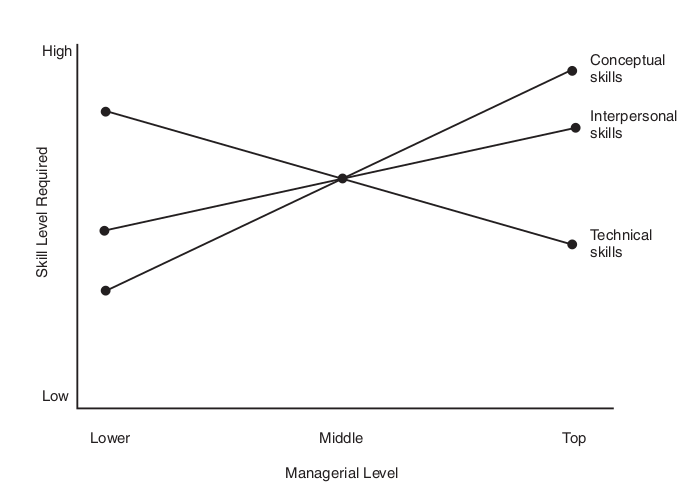
\includegraphics[width=15cm]{managerLevel}
\centering
\end{figure}
% subsection situational_relevance_of_skills (end)

\subsubsection{Evaluation of the Trait Approach} % (fold)
\label{ssub:evaluation_of_the_trait_approach}
Few trait studies include mediating processes to explain why leadership traits and skills are relevant for predicting effectiveness in the current position or career success.
\\Most trait studies are not guided by a theory that explains how traits are related to managerial effectiveness and advancement. Another limitation of the trait approach is the lack of attention in many studies to the leadership context

\begin{center}
\begin{tabular}{ | p{3cm} | p{3cm} | p{3cm}|}
	\\ {\bf Trait } & {\bf Too MUCH} &{\bf  Too LITTLE} \\
	\hline 
	{\bf Self-confidence} & arrogant, acts too quickly, and takes too many risks & indecisive, avoids risks, and does not seek to influence others \\
	\hline
	{\bf Need for Esteem} & preoccupied with reputation and status, exaggerates achievements, covers up mistakes and failures or blames others & does not seek recognition or build a reputation for high expertise and reliability\\
	\hline
	{\bf Need for Affiliation} & overly concerned about being liked and accepted by others, over-uses ingratiation, and will not risk popularity by asking for sacrifices or insisting on better performance & does not try to form strong relationships or build a social support network\\
	\hline
	{\bf Need for Independence} & resents authority, too quick to ignore rules and standard procedures & dependent on others for direction, rule oriented, avoids taking initiative \\
	\hline
	{\bf Altruism (value)} & overly generous and forgiving, unable to ask for sacrifices or maintain discipline & selfish, indifferent about the needs of others, may exploit them for personal gain \\
	\hline
	{\bf Performance Orientation (value)} & the person is a perfectionist and is overly demanding and never satisfied & the person accepts weak performance and does not push for improvement \\
 	\hline
\end{tabular}
\end{center}

\subsubsection{Guidelines for Managers} % (fold)
\label{ssub:guidelines_for_managers}

\begin{itemize}
	\item Learn about your strengths and weaknesses .
	\item Maintain self-awareness .
	\item Identify and develop skills relevant for a future leadership position .
	\item Remember that a strength can become a weakness .
	\item Compensate for weaknesses
\end{itemize}

% subsubsection guidelines_for_managers (end)

\subsubsection{Key Terms} % (fold)
\label{ssub:key_terms}
\begin{itemize}
	\item big five personality traits
	\item cognitive skills
	\item competencies
	\item conceptual skills
	\item derailed careers
	\item emotional intelligence
	\item emotional maturity
	\item emotional stability
	\item interpersonal skills
	\item locus of control orientation
	\item need for achievement
	\item need for affiliation
	\item need for power
	\item personalized power orientation
	\item self-awareness
	\item self-confidence
	\item social intelligence
	\item socialized power orientation
	\item technical skills
\end{itemize}
% subsubsection key_terms (end)

% subsubsection evaluation_of_the_trait_approach (end)